\chapter{REST API Proxy \\
  \small{\textit{-- Author Name}}
  \index{Chapter!rest-api-proxy}
  \label{Chapter::RestApiProxy}}

\section{Forwarding API Requests}
When a REST API request is made to OpenTogetherTube, the request is first received by the load balancer
 acting as the reverse proxy for API requests. The load balancer then selects one of the OTT monoliths based
  on the current load balancing algorithm and forwards the request to the selected monolith. The monolith processes 
  the request and sends a response back to the load balancer acting as the reverse proxy. The load balancer then returns 
  the response to the client that made the original request.

\begin{figure}[!htb]
  \centering
  \scalebox{0.57}{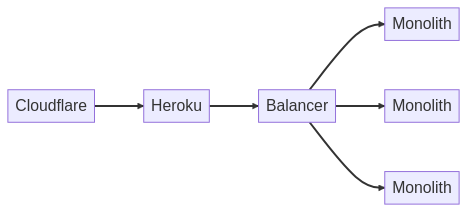
\includegraphics{Figures/api-balancer.png}}
  \caption{\label{Figure::api-balancer} API Balancer Flowchart.}
\end{figure}

\section{Forwarding Requests Credentials}

OpenTogetherTube platform uses tokens to authenticate and authorize users. When a user logs in, the
server generates a token that is stored in the browser's local storage and included in all subsequent requests made
by the user. The server verifies the token to ensure that the user is authenticated and has permission to access the
requested video stream. The token is used to look up the session information in Redis, which allows the server to 
retrieve the user's permissions and session state.